\chapter{Täydellinen haku}

\key{Täydellinen haku}
on yleispätevä tapa ratkaista
lähes mikä tahansa ohjelmointitehtävä.
Ideana on käydä läpi raa'alla voimalla kaikki
mahdolliset tehtävän ratkaisut ja tehtävästä riippuen
valita paras ratkaisu
tai laskea ratkaisuiden yhteismäärä.
          
Täydellinen haku on hyvä menetelmä, jos kaikki
ratkaisut ehtii käydä läpi,
koska haku on yleensä suoraviivainen toteuttaa
ja se antaa varmasti oikean vastauksen.
Jos täydellinen haku on liian hidas,
seuraavien lukujen ahneet algoritmit tai
dynaaminen ohjelmointi voivat soveltua
tehtävään.

\section{Osajoukkojen läpikäynti}

\index{osajoukko@osajoukko}

Joukon osajoukkoja ovat kaikki mahdolliset
tavat valita osa joukon alkioista.
Kun joukossa on $n$ alkiota,
sillä on $2^n$ osajoukkoa.
Esimerkiksi joukon $\{1,2,3\}$
osajoukot ovat $\emptyset$,
$\{1\}$, $\{2\}$, $\{3\}$,
$\{1,2\}$, $\{1,3\}$, $\{2,3\}$ ja $\{1,2,3\}$,
missä $\emptyset$ on tyhjä joukko.

\subsubsection{Menetelmä 1}

Kätevä tapa käydä läpi osajoukot on
käyttää rekursiota.
Seuraava funktio \texttt{haku} muodostaa
joukon $\{1,2,\ldots,n\}$ osajoukot.
Funktio pitää yllä vektoria \texttt{v},
johon se kokoaa osajoukossa olevat luvut.
Osajoukkojen muodostus alkaa
tekemällä funktiokutsu \texttt{haku(1)}.

\begin{lstlisting}
void haku(int k) {
    if (k == n+1) {
        // käsittele osajoukko
    } else {
        haku(k+1);
        v.push_back(k);
        haku(k+1);
        v.pop_back();
    }
}
\end{lstlisting}

Funktion parametri $k$ on luku,
joka on ehdolla lisättäväksi osajoukkoon seuraavaksi.
Joka kutsulla funktio haarautuu kahteen tapaukseen:
joko luku $k$ lisätään tai ei lisätä osajoukkoon.
Aina kun $k=n+1$, kaikki luvut on käyty läpi
ja yksi osajoukko on muodostettu.

Esimerkiksi kun $n=3$, funktion suoritus etenee
seuraavan kuvan mukaisesti.
Joka kutsussa 
vasen haara jättää luvun pois osajoukosta
ja oikea haara lisää sen osajoukkoon.
\begin{center}
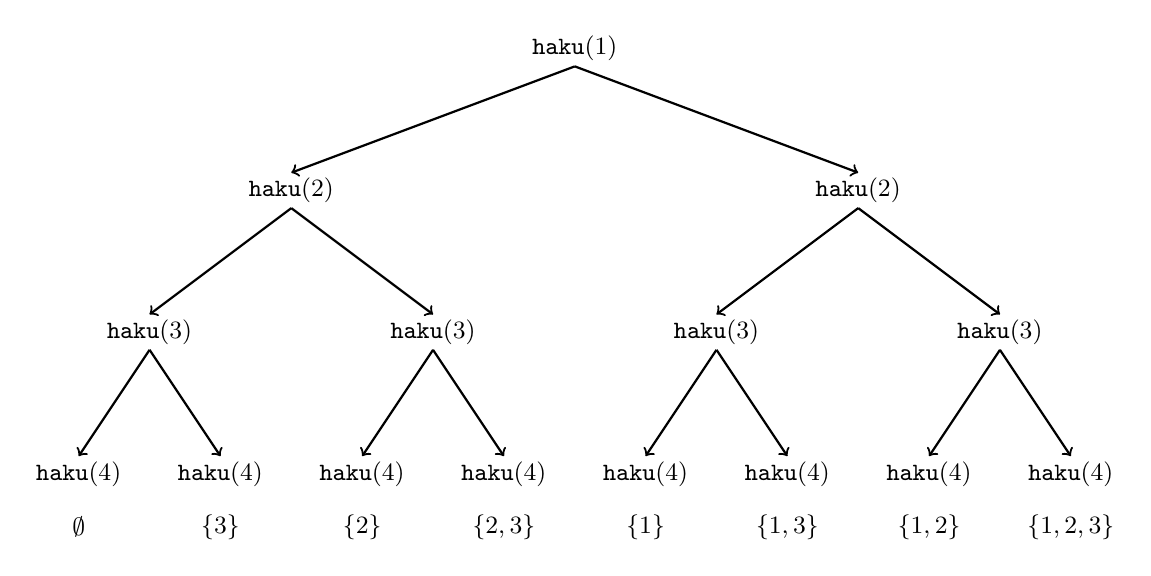
\begin{tikzpicture}[scale=.45]
  \begin{scope}
    \small
    \node at (0,0) {$\texttt{haku}(1)$};

    \node at (-8,-4) {$\texttt{haku}(2)$};
    \node at (8,-4) {$\texttt{haku}(2)$};

    \path[draw,thick,->] (0,0-0.5) -- (-8,-4+0.5);
    \path[draw,thick,->] (0,0-0.5) -- (8,-4+0.5);

    \node at (-12,-8) {$\texttt{haku}(3)$};
    \node at (-4,-8) {$\texttt{haku}(3)$};
    \node at (4,-8) {$\texttt{haku}(3)$};
    \node at (12,-8) {$\texttt{haku}(3)$};

    \path[draw,thick,->] (-8,-4-0.5) -- (-12,-8+0.5);
    \path[draw,thick,->] (-8,-4-0.5) -- (-4,-8+0.5);
    \path[draw,thick,->] (8,-4-0.5) -- (4,-8+0.5);
    \path[draw,thick,->] (8,-4-0.5) -- (12,-8+0.5);

    \node at (-14,-12) {$\texttt{haku}(4)$};
    \node at (-10,-12) {$\texttt{haku}(4)$};
    \node at (-6,-12) {$\texttt{haku}(4)$};
    \node at (-2,-12) {$\texttt{haku}(4)$};
    \node at (2,-12) {$\texttt{haku}(4)$};
    \node at (6,-12) {$\texttt{haku}(4)$};
    \node at (10,-12) {$\texttt{haku}(4)$};
    \node at (14,-12) {$\texttt{haku}(4)$};

    \node at (-14,-13.5) {$\emptyset$};
    \node at (-10,-13.5) {$\{3\}$};
    \node at (-6,-13.5) {$\{2\}$};
    \node at (-2,-13.5) {$\{2,3\}$};
    \node at (2,-13.5) {$\{1\}$};
    \node at (6,-13.5) {$\{1,3\}$};
    \node at (10,-13.5) {$\{1,2\}$};
    \node at (14,-13.5) {$\{1,2,3\}$};


    \path[draw,thick,->] (-12,-8-0.5) -- (-14,-12+0.5);
    \path[draw,thick,->] (-12,-8-0.5) -- (-10,-12+0.5);
    \path[draw,thick,->] (-4,-8-0.5) -- (-6,-12+0.5);
    \path[draw,thick,->] (-4,-8-0.5) -- (-2,-12+0.5);
    \path[draw,thick,->] (4,-8-0.5) -- (2,-12+0.5);
    \path[draw,thick,->] (4,-8-0.5) -- (6,-12+0.5);
    \path[draw,thick,->] (12,-8-0.5) -- (10,-12+0.5);
    \path[draw,thick,->] (12,-8-0.5) -- (14,-12+0.5);
\end{scope}
\end{tikzpicture}
\end{center}

\subsubsection{Menetelmä 2}

Toinen tapa käydä osajoukot läpi on hyödyntää kokonaislukujen
bittiesitystä. Jokainen $n$ alkion osajoukko
voidaan esittää $n$ bitin jonona,
joka taas vastaa lukua väliltä $0 \ldots 2^n-1$.
Bittiesityksen ykkösbitit ilmaisevat,
mitkä joukon alkiot on valittu osajoukkoon.

Tarkastellaan esimerkiksi joukkoa $\{1,2,3,4,5\}$.
Nyt jokaista joukon osajoukkoa vastaa jokin
5 bitin jono.
Esimerkiksi osajoukon $\{2,3,5\}$ bittiesitys on 01101,
jossa bitit 1 ja 4 ovat nollia
ja bitit 2, 3, ja 5 ovat ykkösiä.

Seuraava koodi käy läpi $n$ alkion joukon
osajoukkojen bittiesitykset:

\begin{lstlisting}
for (int b = 0; b < (1<<n); b++) {
    // käsittele osajoukko b
}
\end{lstlisting}

Seuraava koodi muodostaa jokaisen osajoukon
kohdalla vektorin \texttt{v},
joka sisältää osajoukossa olevat luvut.
Ne saadaan selville tutkimalla, mitkä bitit ovat
ykkösiä osajoukon bittiesityksessä.

\begin{lstlisting}
for (int b = 0; b < (1<<n); b++) {
    vector<int> v;
    for (int i = 0; i < n; i++) {
        if (b&(1<<i)) v.push_back(i+1);
    }
}
\end{lstlisting}

\section{Permutaatioiden läpikäynti}

\index{permutaatio@permutaatio}

Joukon permutaatiot ovat alkioiden mahdolliset
järjestykset.
Kun joukossa on $n$ alkiota,
permutaatioita on kaikkiaan $n!$.
Esimerkiksi joukon $\{1,2,3\}$
permutaatiot ovat $(1,2,3)$, $(1,3,2)$,
$(2,1,3)$, $(2,3,1)$, $(3,1,2)$ ja $(3,2,1)$.

\subsubsection{Menetelmä 1}

Osajoukkojen tavoin permutaatioita voi muodostaa
rekursiivisesti.
Seuraava funktio \texttt{haku} käy läpi
joukon $\{1,2,\ldots,n\}$ permutaatiot.
Funktio muodostaa kunkin permutaation
vuorollaan vektoriin \texttt{v}.
Permutaatioiden muodostus alkaa kutsumalla
funktiota ilman parametreja.

\begin{lstlisting}
void haku() {
    if (v.size() == n) {
        // käsittele permutaatio
    } else {
        for (int i = 1; i <= n; i++) {
            if (p[i]) continue;
            p[i] = 1;
            v.push_back(i);
            haku();
            p[i] = 0;
            v.pop_back();
        }
    }
}
\end{lstlisting}

Funktion jokainen kutsu lisää uuden
luvun permutaatioon vektoriin \texttt{v}.
Taulukko \texttt{p} kertoo, mitkä luvut on jo
valittu permutaatioon.
Jos $\texttt{p}[k]=0$, luku $k$ ei ole mukana,
ja jos $\texttt{p}[k]=1$, luku $k$ on mukana.
Jos vektorin \texttt{v} koko on sama kuin
joukon koko $n$, permutaatio on tullut valmiiksi.

\subsubsection{Menetelmä 2}

\index{next\_permutation@\texttt{next\_permutation}}

Vaihtoehtoinen tapa käydä läpi permutaatiot
on käyttää C++:n standardikirjastoon kuuluvaa
funktiota \texttt{next\_permutation}.
Se muuttaa taulukossa olevan permutaation
seuraavaksi järjestyksessä olevaksi permutaatioksi.

Seuraava koodi muodostaa joukon $\{1,2,\ldots,n\}$
permutaatiot käyttäen apuna funktiota \texttt{next\_permutation}:

\begin{lstlisting}
vector<int> v;
for (int i = 1; i <= n; i++) {
    v.push_back(i);
}
do {
    // käsittele permutaatio
} while (next_permutation(v.begin(),v.end()));
\end{lstlisting}

\section{Peruuttava haku}

\index{peruuttava haku@peruuttava haku}

\key{Peruuttava haku}
aloittaa ratkaisun etsimisen tyhjästä
ja laajentaa ratkaisua askel kerrallaan.
Joka askeleella haku haarautuu kaikkiin
mahdollisiin suuntiin, joihin ratkaisua voi laajentaa.
Haaran tutkimisen jälkeen haku peruuttaa takaisin
ja jatkaa muihin mahdollisiin suuntiin.

Tarkastellaan esimerkkinä seuraavaa tehtävää:

\begin{task}
Montako tapaa on asettaa $n$ kuningatarta
$n \times n$ -shakkilaudalle niin,
että mitkään kaksi kuningatarta eivät uhkaa toisiaan?
\end{task}

Esimerkiksi kun $n=4$, mahdolliset ratkaisut ovat seuraavat:

\begin{center}
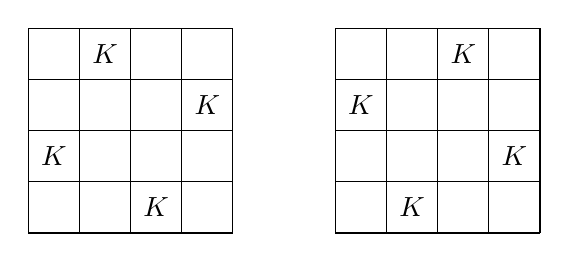
\begin{tikzpicture}[scale=.65]
  \begin{scope}
    \draw (0, 0) grid (4, 4);
    \node at (1.5,3.5) {$K$};
    \node at (3.5,2.5) {$K$};
    \node at (0.5,1.5) {$K$};
    \node at (2.5,0.5) {$K$};

    \draw (6, 0) grid (10, 4);
    \node at (6+2.5,3.5) {$K$};
    \node at (6+0.5,2.5) {$K$};
    \node at (6+3.5,1.5) {$K$};
    \node at (6+1.5,0.5) {$K$};

  \end{scope}
\end{tikzpicture}
\end{center}

Tehtävän voi ratkaista peruuttavalla haulla
muodostamalla ratkaisua rivi kerrallaan.
Jokaisella rivillä täytyy valita yksi ruuduista,
johon sijoitetaan kuningatar niin,
ettei se uhkaa mitään aiemmin lisättyä kuningatarta.
Ratkaisu on valmis, kun viimeisellekin
riville on lisätty kuningatar.

Esimerkiksi kun $n=4$, osa peruuttavan haun muodostamasta
puusta näyttää seuraavalta:

\begin{center}
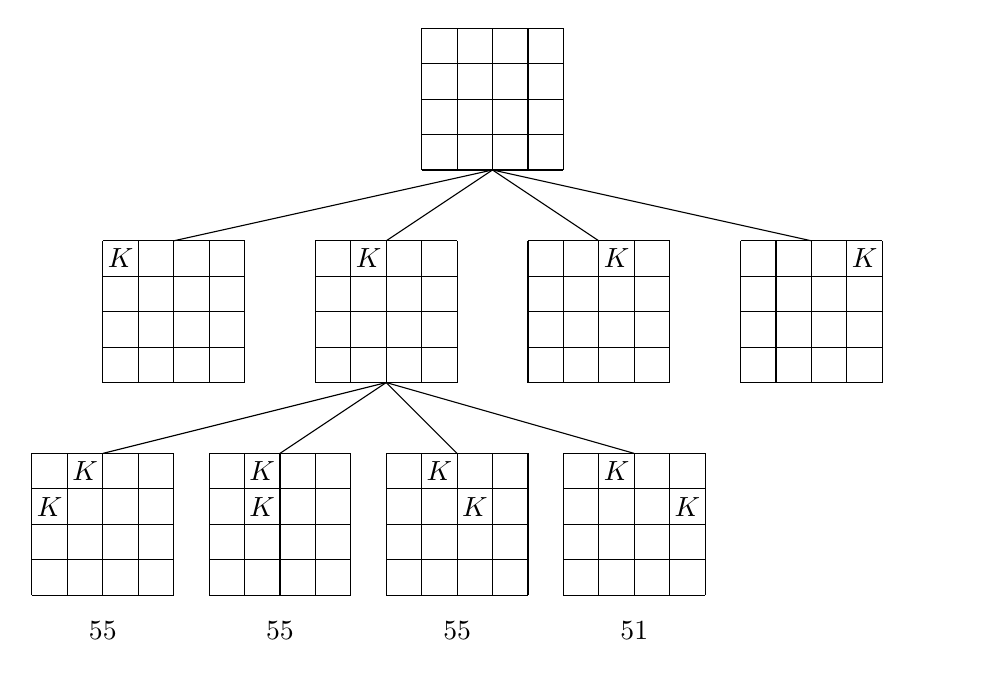
\begin{tikzpicture}[scale=.45]
  \begin{scope}
    \draw (0, 0) grid (4, 4);

    \draw (-9, -6) grid (-5, -2);
    \draw (-3, -6) grid (1, -2);
    \draw (3, -6) grid (7, -2);
    \draw (9, -6) grid (13, -2);

    \node at (-9+0.5,-3+0.5) {$K$};
    \node at (-3+1+0.5,-3+0.5) {$K$};
    \node at (3+2+0.5,-3+0.5) {$K$};
    \node at (9+3+0.5,-3+0.5) {$K$};

    \draw (2,0) -- (-7,-2);
    \draw (2,0) -- (-1,-2);
    \draw (2,0) -- (5,-2);
    \draw (2,0) -- (11,-2);

    \draw (-11, -12) grid (-7, -8);
    \draw (-6, -12) grid (-2, -8);
    \draw (-1, -12) grid (3, -8);
    \draw (4, -12) grid (8, -8);
    \draw[white] (11, -12) grid (15, -8);
    \node at (-11+1+0.5,-9+0.5) {$K$};
    \node at (-6+1+0.5,-9+0.5) {$K$};
    \node at (-1+1+0.5,-9+0.5) {$K$};
    \node at (4+1+0.5,-9+0.5) {$K$};
    \node at (-11+0+0.5,-10+0.5) {$K$};
    \node at (-6+1+0.5,-10+0.5) {$K$};
    \node at (-1+2+0.5,-10+0.5) {$K$};
    \node at (4+3+0.5,-10+0.5) {$K$};

    \draw (-1,-6) -- (-9,-8);
    \draw (-1,-6) -- (-4,-8);
    \draw (-1,-6) -- (1,-8);
    \draw (-1,-6) -- (6,-8);

    \node at (-9,-13) {\ding{55}};
    \node at (-4,-13) {\ding{55}};
    \node at (1,-13) {\ding{55}};
    \node at (6,-13) {\ding{51}};

  \end{scope}
\end{tikzpicture}
\end{center}

Kuvan alimmalla tasolla kolme ensimmäistä osaratkaisua
eivät kelpaa, koska niissä kuningattaret uhkaavat
toisiaan.
Sen sijaan neljäs osaratkaisu kelpaa,
ja sitä on mahdollista laajentaa loppuun asti
kokonaiseksi ratkaisuksi.

\begin{samepage}
Seuraava koodi toteuttaa peruuttavan haun:

\begin{lstlisting}
void haku(int y) {
    if (y == n) {
        c++;
        return;
    }
    for (int x = 0; x < n; x++) {
        if (xx[x] || d1[x+y] || d2[x-y+n-1]) continue;
        xx[x] = d1[x+y] = d2[x-y+n-1] = 1;
        haku(y+1);
        xx[x] = d1[x+y] = d2[x-y+n-1] = 0;
    }
}
\end{lstlisting}
\end{samepage}
Haku alkaa kutsumalla funktiota \texttt{haku(0)}.
Laudan koko on muuttujassa $n$,
ja koodi laskee ratkaisuiden määrän
muuttujaan $c$.

Koodi olettaa, että laudan vaaka- ja pystyrivit
on numeroitu 0:sta alkaen.
Funktio asettaa kuningattaren vaakariville $y$,
kun $0 \le y < n$.
Jos taas $y=n$, yksi ratkaisu on valmis
ja funktio kasvattaa muuttujaa $c$.

Taulukko \texttt{xx} pitää kirjaa,
millä laudan pystyriveillä on jo kuningatar.
Vastaavasti taulukot \texttt{d1} ja \texttt{d2}
pitävät kirjaa vinoriveistä.
Tällaisille riveille ei voi laittaa enää toista
kuningatarta.
Esimerkiksi $4 \times 4$ -laudan tapauksessa
vinorivit on numeroitu seuraavasti:

\begin{center}
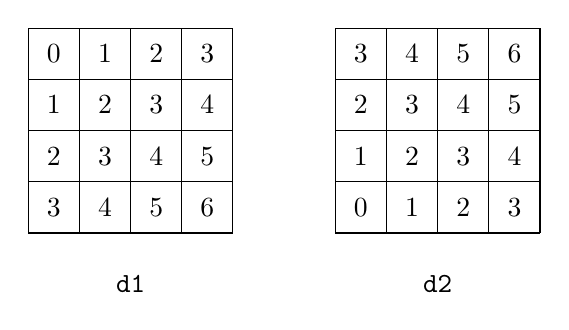
\begin{tikzpicture}[scale=.65]
  \begin{scope}
    \draw (0, 0) grid (4, 4);
    \node at (0.5,3.5) {$0$};
    \node at (1.5,3.5) {$1$};
    \node at (2.5,3.5) {$2$};
    \node at (3.5,3.5) {$3$};
    \node at (0.5,2.5) {$1$};
    \node at (1.5,2.5) {$2$};
    \node at (2.5,2.5) {$3$};
    \node at (3.5,2.5) {$4$};
    \node at (0.5,1.5) {$2$};
    \node at (1.5,1.5) {$3$};
    \node at (2.5,1.5) {$4$};
    \node at (3.5,1.5) {$5$};
    \node at (0.5,0.5) {$3$};
    \node at (1.5,0.5) {$4$};
    \node at (2.5,0.5) {$5$};
    \node at (3.5,0.5) {$6$};

    \draw (6, 0) grid (10, 4);
    \node at (6.5,3.5) {$3$};
    \node at (7.5,3.5) {$4$};
    \node at (8.5,3.5) {$5$};
    \node at (9.5,3.5) {$6$};
    \node at (6.5,2.5) {$2$};
    \node at (7.5,2.5) {$3$};
    \node at (8.5,2.5) {$4$};
    \node at (9.5,2.5) {$5$};
    \node at (6.5,1.5) {$1$};
    \node at (7.5,1.5) {$2$};
    \node at (8.5,1.5) {$3$};
    \node at (9.5,1.5) {$4$};
    \node at (6.5,0.5) {$0$};
    \node at (7.5,0.5) {$1$};
    \node at (8.5,0.5) {$2$};
    \node at (9.5,0.5) {$3$};

    \node at (2,-1) {\texttt{d1}};
    \node at (8,-1) {\texttt{d2}};

  \end{scope}
\end{tikzpicture}
\end{center}

Koodin avulla selviää esimerkiksi,
että tapauksessa $n=8$ on 92 tapaa sijoittaa 8
kuningatarta $8 \times 8$ -laudalle.
Kun $n$ kasvaa, koodi hidastuu nopeasti,
koska ratkaisujen määrä kasvaa räjähdysmäisesti.
Tapauksen $n=16$ laskeminen vie jo noin minuutin
nykyaikaisella tietokoneella (14772512 ratkaisua).

\section{Haun optimointi}

Peruuttavaa hakua on usein mahdollista tehostaa
huomattavasti erilaisten optimointien avulla.
Tarkastellaan esimerkkinä seuraavaa tehtävää:

\begin{task}
Aloitat $n \times n$ -ruudukon
vasemmasta yläkulmasta ja tehtäväsi on päästä
oikeaan alakulmaan.
Saat liikkua joka vuorolla askeleen
ylöspäin, alaspäin, vasemmalle tai oikealle.
Sinun tulee käydä reitin aikana tasan kerran
kussakin ruudussa.
Montako erilaista reittiä on olemassa?
\end{task}

Esimerkiksi $7 \times 7$ -ruudukossa on
111712 mahdollista reittiä vasemmasta yläkulmasta
oikeaan alakulmaan, joista yksi on seuraava:

\begin{center}
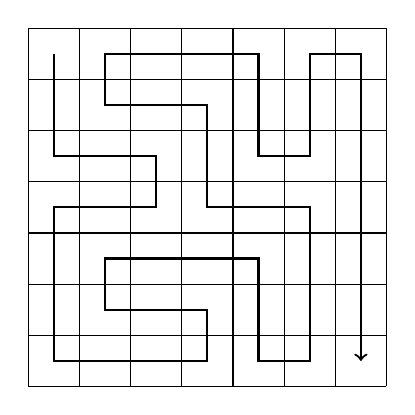
\begin{tikzpicture}[scale=.65]
  \begin{scope}
    \draw (0, 0) grid (7, 7);
    \draw[thick,->] (0.5,6.5) -- (0.5,4.5) -- (2.5,4.5) --
          (2.5,3.5) -- (0.5,3.5) -- (0.5,0.5) --
          (3.5,0.5) -- (3.5,1.5) -- (1.5,1.5) --
          (1.5,2.5) -- (4.5,2.5) -- (4.5,0.5) --
          (5.5,0.5) -- (5.5,3.5) -- (3.5,3.5) --
          (3.5,5.5) -- (1.5,5.5) -- (1.5,6.5) --
          (4.5,6.5) -- (4.5,4.5) -- (5.5,4.5) --
          (5.5,6.5) -- (6.5,6.5) -- (6.5,0.5);
  \end{scope}
\end{tikzpicture}
\end{center}

Keskitymme seuraavaksi nimenomaan tapaukseen $7 \times 7$,
koska se on laskennallisesti sopivan haastava.
Lähdemme liikkeelle suoraviivaisesta peruuttavaa hakua
käyttävästä algoritmista
ja teemme siihen pikkuhiljaa optimointeja,
jotka nopeuttavat hakua eri tavoin.

Mittaamme jokaisen optimoinnin jälkeen
algoritmin suoritusajan sekä rekursiokutsujen yhteismäärän,
jotta näemme selvästi, mikä vaikutus kullakin
optimoinnilla on haun tehokkuuteen.

\subsubsection{Algoritmi}

Algoritmin ensimmäisessä versiossa ei ole mitään optimointeja,
vaan peruuttava haku käy läpi kaikki mahdolliset tavat
muodostaa reitti ruudukon vasemmasta yläkulmasta
oikeaan alakulmaan.

\begin{itemize}
\item
suoritusaika: 483 sekuntia
\item
rekursiokutsuja: 76 miljardia
\end{itemize}

\subsubsection{Optimointi 1}

Reitin ensimmäinen askel on joko alaspäin
tai oikealle. Tästä valinnasta seuraavat tilanteet
ovat symmetrisiä ruudukon lävistäjän suhteen.
Niinpä voimme mennä aina ensin alaspäin
ja kertoa lopuksi reittien määrä 2:lla.

\begin{itemize}
\item
suoritusaika: 244 sekuntia
\item
rekursiokutsuja: 38 miljardia
\end{itemize}

\subsubsection{Optimointi 2}

Jos reitti menee oikean alakulman ruutuun ennen kuin
se on käynyt kaikissa muissa ruuduissa,
siitä ei voi mitenkään enää saada kelvollista ratkaisua.
Niinpä voimme hylätä haun aikana kaikki tällaiset reitit.

\begin{itemize}
\item
suoritusaika: 119 sekuntia
\item
rekursiokutsuja: 20 miljardia
\end{itemize}

\subsubsection{Optimointi 3}

Jos reitti osuu seinään niin, että kummallakin puolella
on ruutu, jossa reitti ei ole vielä käynyt,
ruudukko jakautuu kahteen osaan.
Näin on esimerkiksi seuraavassa tilanteessa:

\begin{center}
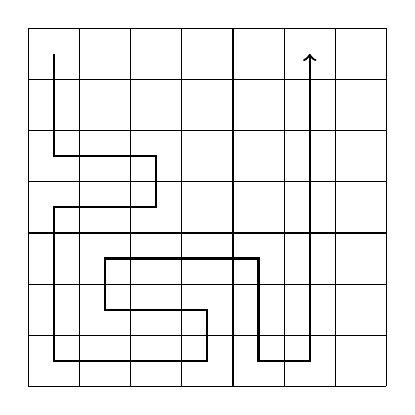
\begin{tikzpicture}[scale=.65]
  \begin{scope}
    \draw (0, 0) grid (7, 7);
    \draw[thick,->] (0.5,6.5) -- (0.5,4.5) -- (2.5,4.5) --
          (2.5,3.5) -- (0.5,3.5) -- (0.5,0.5) --
          (3.5,0.5) -- (3.5,1.5) -- (1.5,1.5) --
          (1.5,2.5) -- (4.5,2.5) -- (4.5,0.5) --
          (5.5,0.5) -- (5.5,6.5);
  \end{scope}
\end{tikzpicture}
\end{center}

Nyt ei ole enää mahdollista käydä kaikissa ruuduissa,
joten voimme hylätä kaikki tällaiset reitit.
Tämä optimointi on hyvin hyödyllinen:

\begin{itemize}
\item
suoritusaika: 1{,}8 sekuntia
\item
rekursiokutsuja: 221 miljoonaa
\end{itemize}

\subsubsection{Optimointi 4}

Äskeisen optimoinnin ideaa voi yleistää:
jos nykyisen ruudun ylä- ja alapuolella on
seinä tai aiemmin käyty ruutu
sekä vasemmalla ja oikealla on
vielä käymätön ruutu (tai päinvastoin),
voimme hylätä reitin.

\begin{itemize}
\item
suoritusaika: 0{,}6 sekuntia
\item
rekursiokutsuja: 69 miljoonaa
\end{itemize}

~\\
Nyt on hyvä hetki lopettaa optimointi ja muistella,
mistä lähdimme liikkeelle.
Alkuperäinen algoritmi vei aikaa 483 sekuntia,
ja nyt optimointien jälkeen algoritmi vie aikaa
vain 0{,}6 sekuntia.
Optimointien ansiosta algoritmin nopeutui
siis lähes 1000-kertaisesti.

Tämä on yleinen ilmiö peruuttavassa haussa,
koska hakupuu on yleensä valtava ja
yksinkertainenkin optimointi voi karsia suuren
määrän haaroja hakupuusta.
Erityisen hyödyllisiä ovat optimoinnit,
jotka kohdistuvat hakupuun yläosaan,
koska ne karsivat eniten haaroja.

\section{Puolivälihaku}

\index{puolivxlihaku@puolivälihaku}

\key{Puolivälihaku} (''meet in the middle'') on tekniikka,
jossa hakutehtävä jaetaan kahteen yhtä suureen osaan.
Kumpaankin osaan tehdään erillinen haku,
ja lopuksi hakujen tulokset yhdistetään.
Puolivälihaun hyötynä on, että sen avulla voi
parantaa haun aikavaativuutta.

\begin{samepage}
Tutustumme puolivälihakuun seuraavan tehtävän kautta:
\begin{task}
Annettuna on lista, jossa on $n$ lukua,
sekä lisäksi kokonaisluku $x$.
Tehtäväsi on selvittää, voiko listan luvuista
valita osajoukon niin, että osajoukon lukujen summa on $x$.
\end{task}
\end{samepage}

Tavanomainen ratkaisu tehtävään on käydä kaikki
listan alkioiden osajoukot läpi ja tarkastaa,
onko jonkin osajoukon summa $x$.
Tällainen ratkaisu kuluttaa aikaa $O(2^n)$,
koska erilaisia osajoukkoja on $2^n$.
Puolivälihaun avulla on kuitenkin mahdollista luoda
tehokkaampi $O(2^{n/2})$-aikainen ratkaisu.

Ideana on jakaa syötteenä oleva lista
kahteen listaan $A$ ja $B$,
joista kumpikin sisältää noin puolet alkioista.
Ensimmäinen haku muodostaa kaikki osajoukot
listan $A$ luvuista ja laittaa muistiin niiden summat
listaan $S_A$.
Toinen haku käsittelee vastaavasti listan $B$ luvut
ja laittaa niiden summat listaan $S_B$.
Tämän jälkeen riittää tarkastaa,
onko mahdollista valita yksi luku listasta $S_A$
ja toinen luku listasta $S_B$ niin,
että lukujen summa on $x$.
Tämän on mahdollista tarkalleen silloin,
kun alkuperäisen listan luvuista saa summan $x$.

Tarkastellaan esimerkkiä,
jossa lista on $\{2,4,5,9\}$
ja $x=15$.
Puolivälihaku muodostaa listat $A=\{2,4\}$
ja $B=\{5,9\}$ sekä summalistat
$S_A=\{0,2,4,6\}$ ja $S_B=\{0,5,9,14\}$.
Summa $x=15$ on mahdollista muodostaa,
koska voidaan valita $S_A$:sta luku $6$
ja $S_B$:stä luku $9$.
Tämä vastaa ratkaisua $\{2,4,9\}$.

Ratkaisun aikavaativuus on huolellisesti toteutettuna
vain $O(2^{n/2})$.
Listat $S_A$ ja $S_B$ on kumpikin mahdollista
muodostaa ajassa $O(2^{n/2})$ niin,
että niiden luvut ovat järjestyksessä.
Tämän jälkeen on mahdollista tutkia ajassa
$O(2^{n/2})$, voiko lukua $x$ muodostaa
valitsemalla kummastakin listasta yksi luku.

Vaikka aikavaativuudet $O(2^n)$ ja $O(2^{n/2})$
muistuttavat toisiaan, niiden ero on merkittävä.
Vakiokertoimilla \emph{on} siis väliä, jos ne esiintyvät
potenssin eksponentissa.
Esimerkiksi jos $n=40$, $O(2^n)$-algoritmin suoritus
veisi tunteja aikaa, kun taas $O(2^{n/2})$
valmistuu sekunnin murto-osassa.


